\subsection{On the mehcanism of modes $A'$ and $QS$}

\begin{figure}
  \centering
  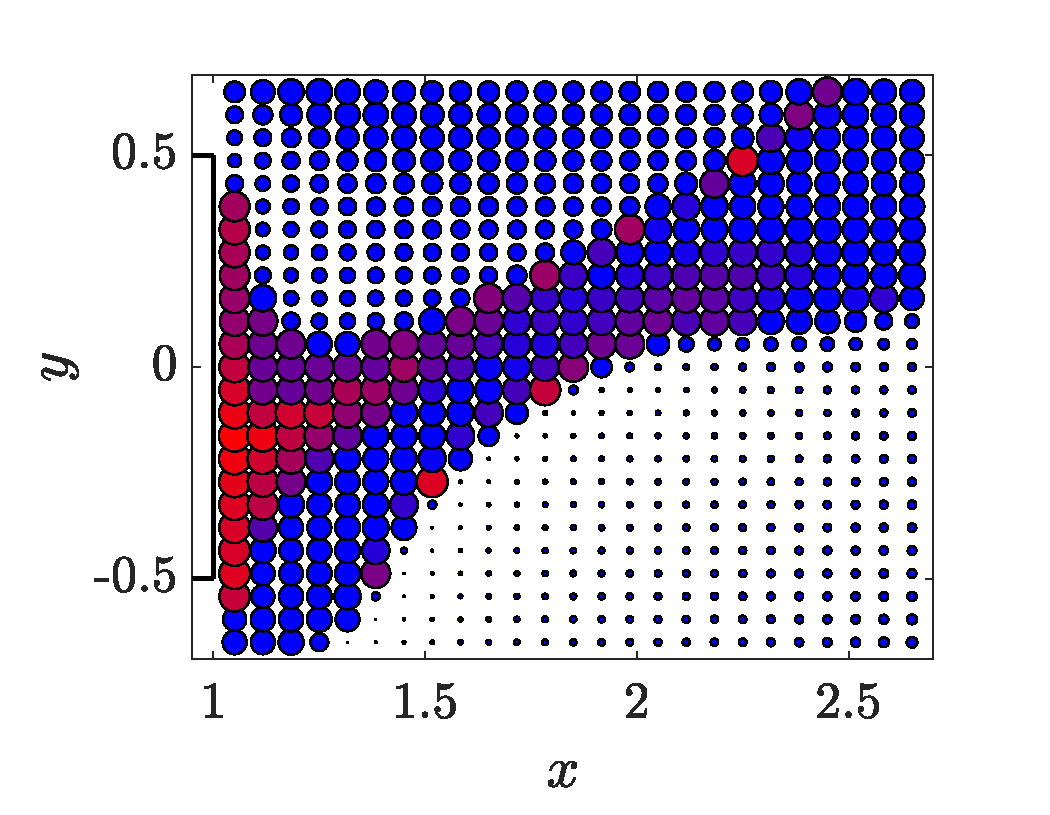
\includegraphics[width=0.49\textwidth]{./fig/LagTrac/part_AR1_Re200.eps}
  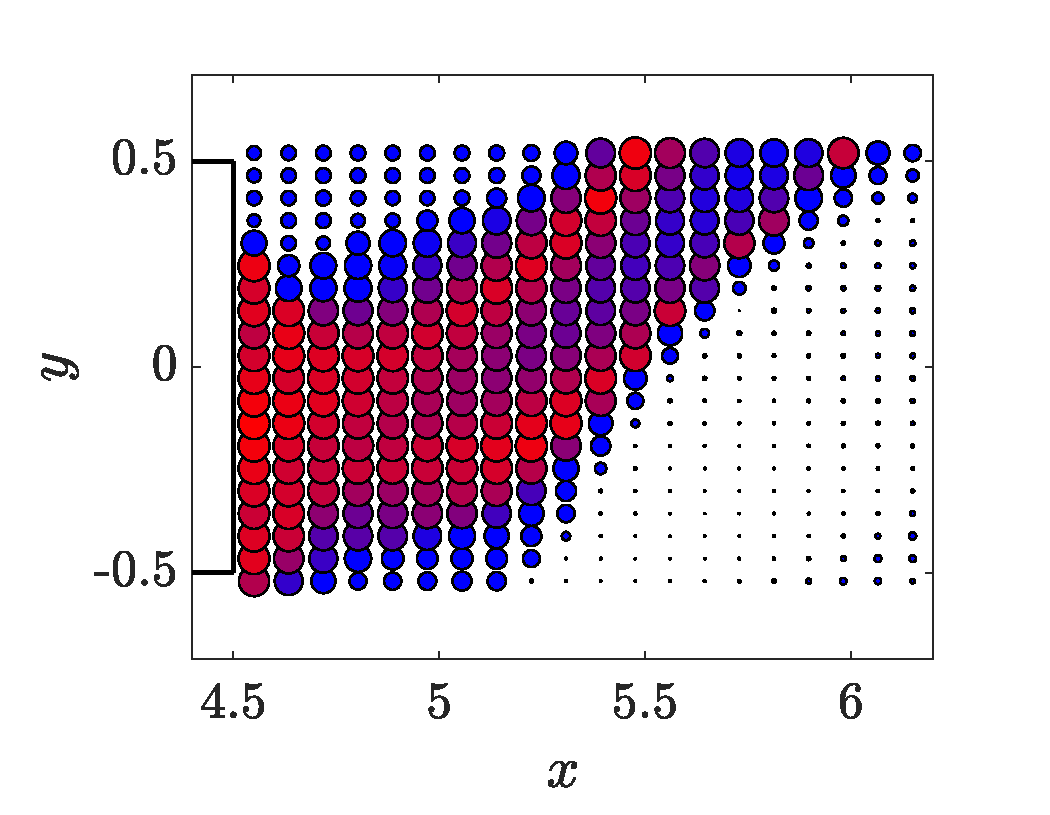
\includegraphics[width=0.49\textwidth]{./fig/LagTrac/part_AR4p5_Re410.eps}
  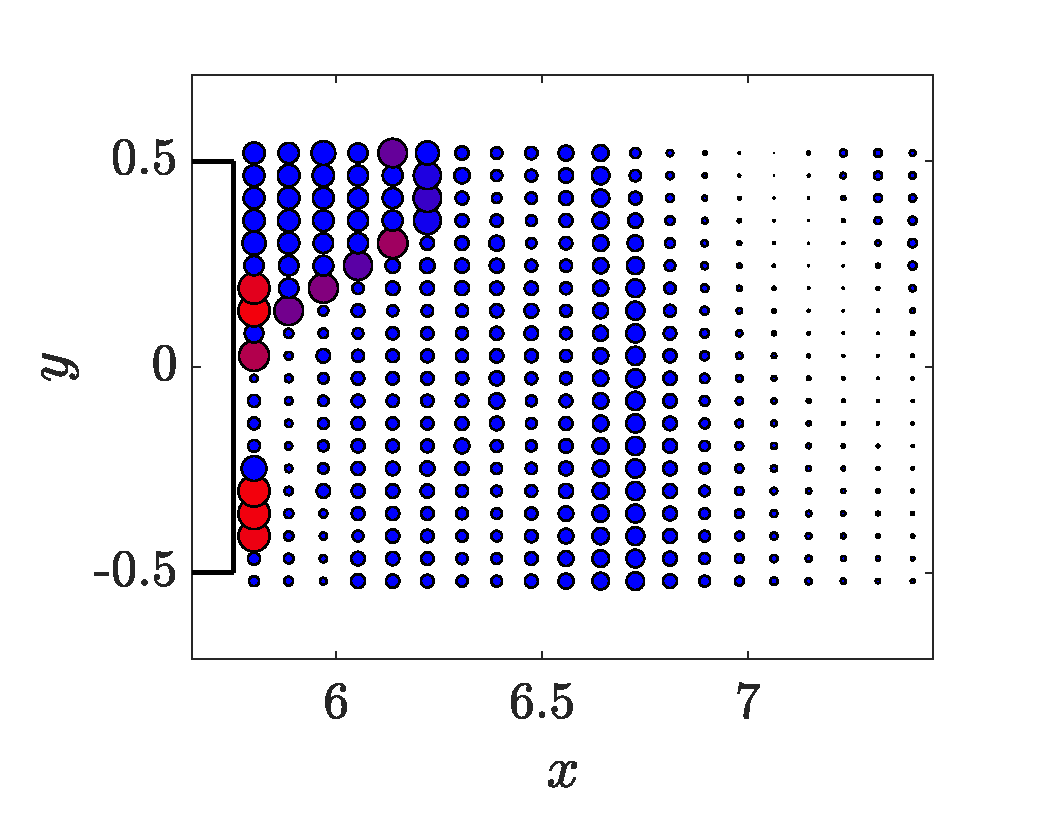
\includegraphics[width=0.49\textwidth]{./fig/LagTrac/part_AR5p75_Re550.eps}
  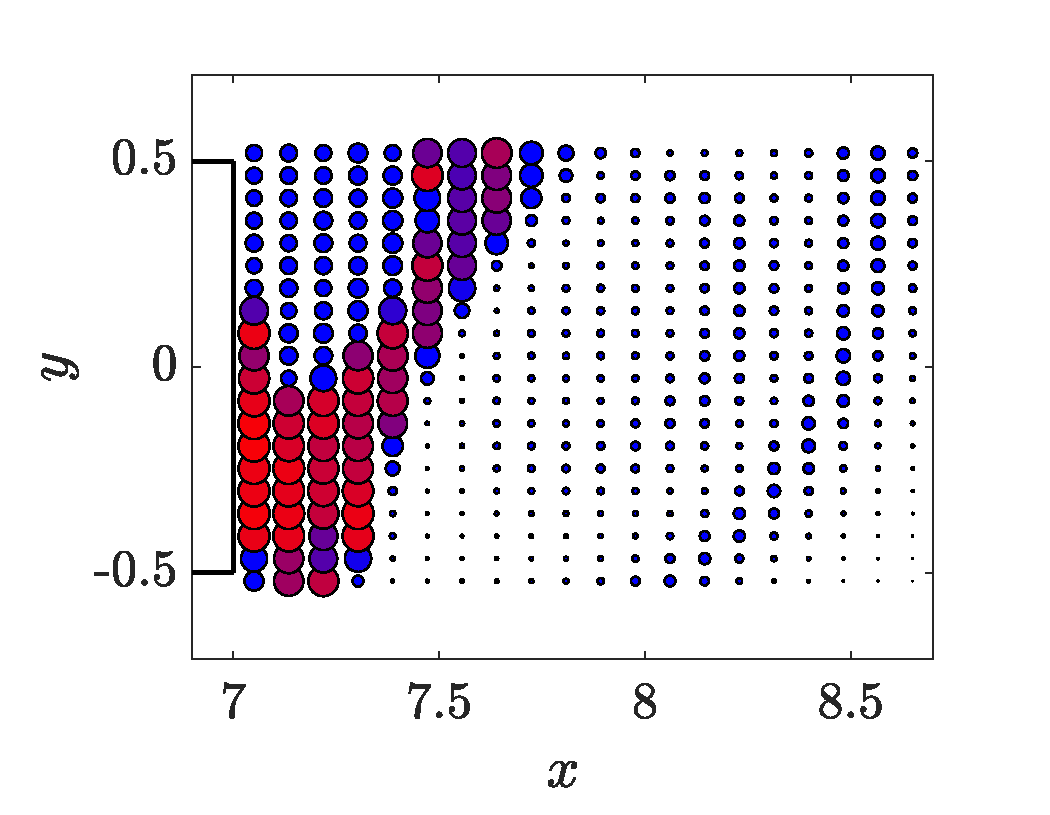
\includegraphics[width=0.49\textwidth]{./fig/LagTrac/part_AR7_Re500.eps}  
  \caption{XX AUMENTARE IL RANGE INVESTIGATO XX}
  \label{fig:part_res}
\end{figure}    

\begin{figure}
  \centering
  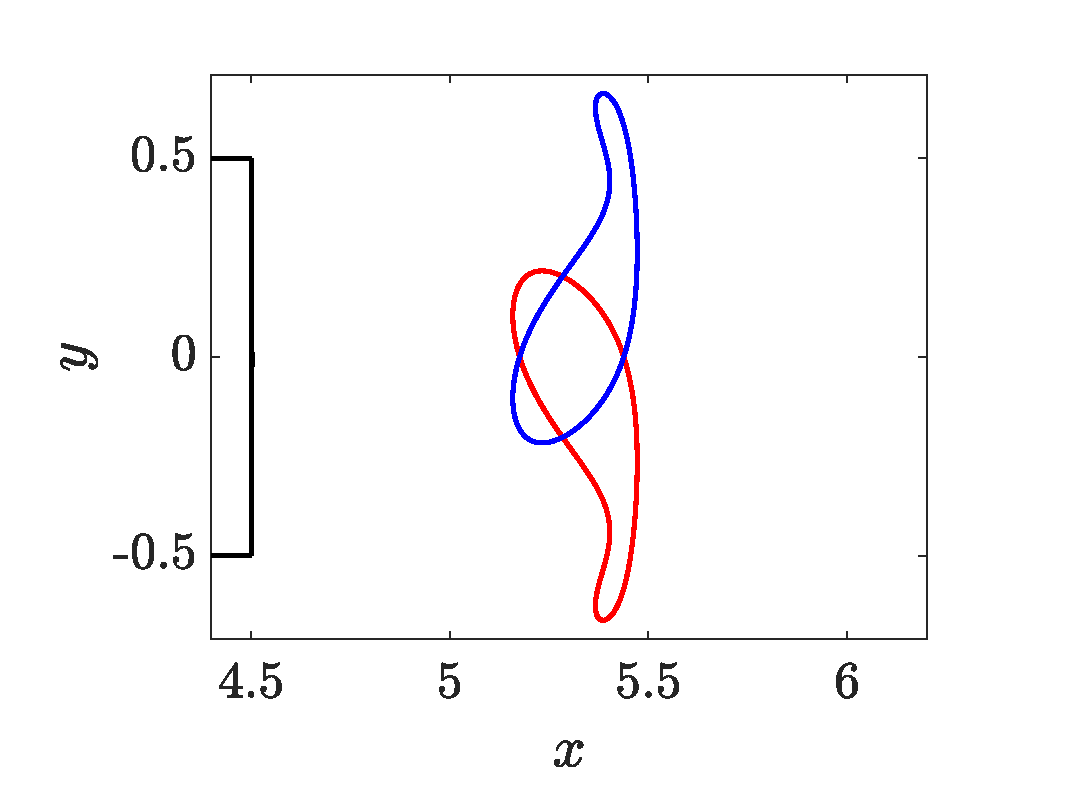
\includegraphics[width=0.49\textwidth]{./fig/LagTrac/orb_AR4p5_Re410.eps}   
  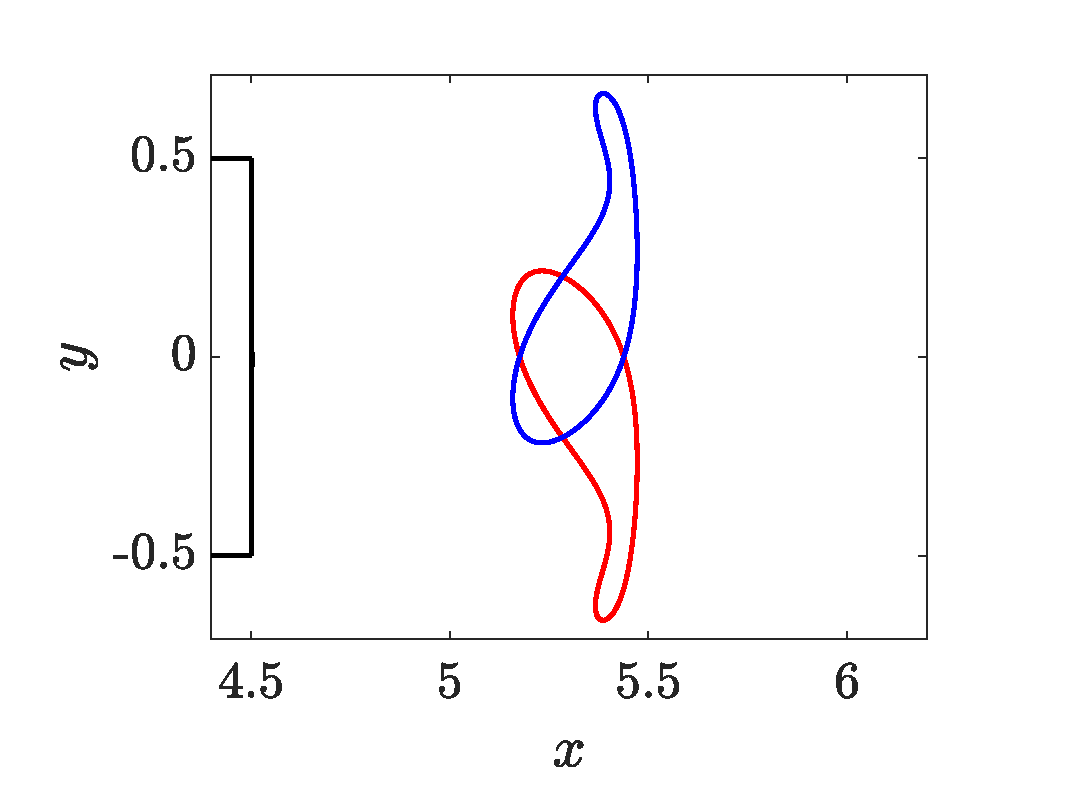
\includegraphics[width=0.49\textwidth]{./fig/LagTrac/orb_AR4p5_Re410.eps} 
  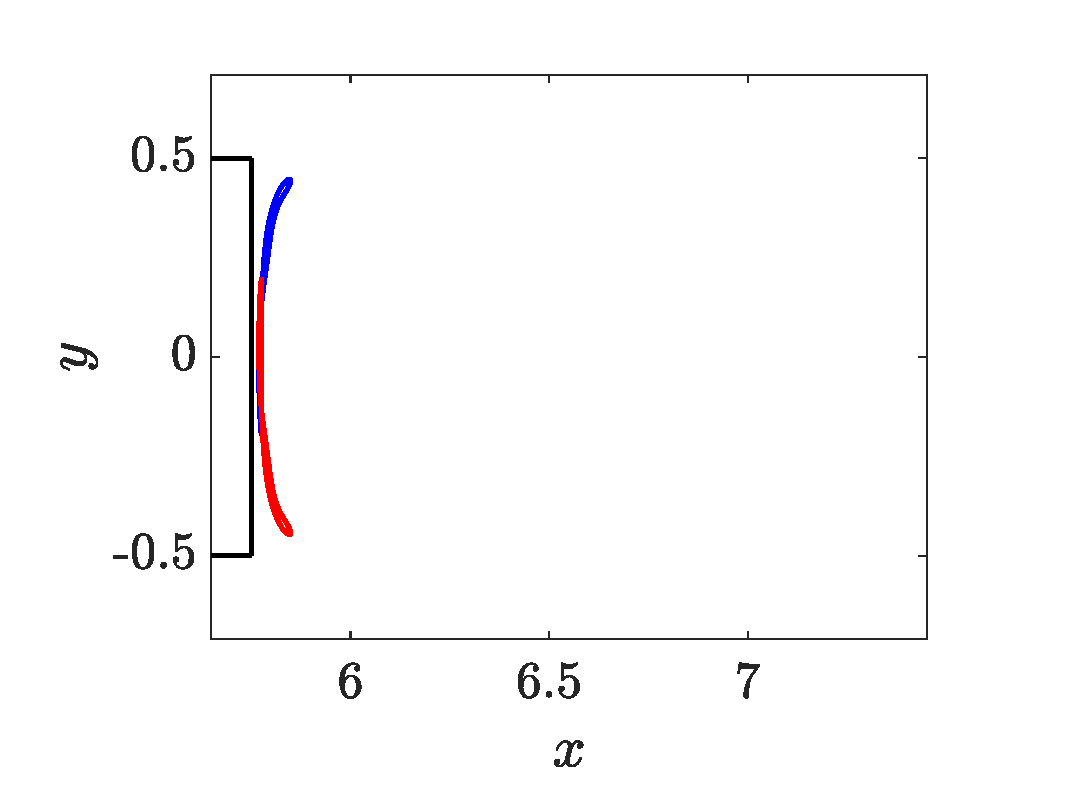
\includegraphics[width=0.49\textwidth]{./fig/LagTrac/orb_AR5p75_Re550.eps}
  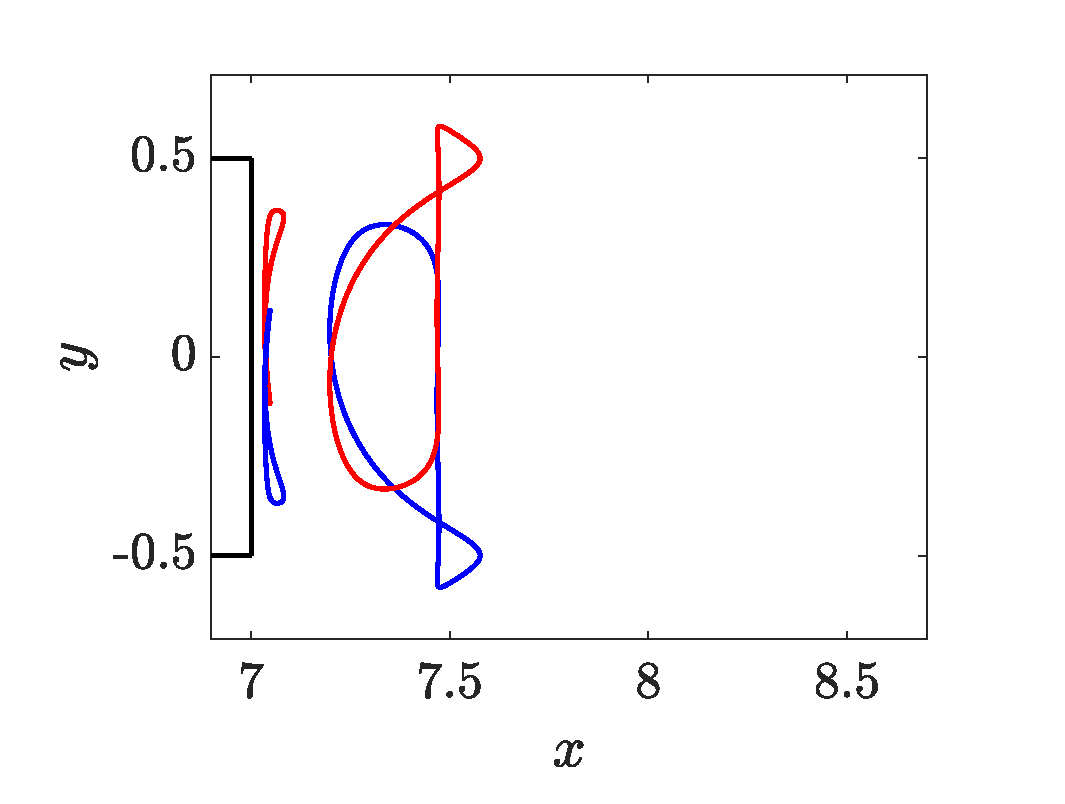
\includegraphics[width=0.49\textwidth]{./fig/LagTrac/orb_AR7_Re500.eps}
  \caption{XX AUMENTARE IL RANGE INVESTIGATO XX}
  \label{fig:part_res}
\end{figure}
